%%%%%%%%%%%%%%%%%%%%%%%%%%%%%%%%%%%%%%%%%%%%%%%%%%%%%%%%%%%%%%%%%%%%%%%%%%%%
%%%%%                          GLOSSAIRE                              %%%%%%
%%%%%%%%%%%%%%%%%%%%%%%%%%%%%%%%%%%%%%%%%%%%%%%%%%%%%%%%%%%%%%%%%%%%%%%%%%%%

\phantomsection 
\addcontentsline{toc}{chapter}{Confusing concepts - Disambiguation} \mtcaddchapter
\label{Ann:gloss}
\addtocontents{toc}{\protect\addvspace{10pt}}

\vspace*{-1.6cm}
\begin{flushright}
\section*{\fontsize{20pt}{20pt}\selectfont\textnormal{Confusing concepts - Disambiguation}}
\end{flushright}
\vspace{-0.2cm}


\lhead[\fancyplain{}{Confusing concepts - Disambiguation}]
      {\fancyplain{}{}}
\chead[\fancyplain{}{}]
      {\fancyplain{}{}}
\rhead[\fancyplain{}{}]
      {\fancyplain{}{Confusing concepts - Disambiguation}}
\lfoot[\fancyplain{}{}]
      {\fancyplain{}{}}
\cfoot[\fancyplain{}{\thepage}]
      {\fancyplain{}{\thepage}}
\rfoot[\fancyplain{}{}]%
     {\fancyplain{}{\scriptsize}}

%%%%%%%%%%%%%%%%%%%%%%%%%%%%%%%%%%%%%%%%%%%%%%%%%%%%%%%%%%%%%%%%%%%%%%%%%%
%%%%%                      Start part here                          %%%%%%
%%%%%%%%%%%%%%%%%%%%%%%%%%%%%%%%%%%%%%%%%%%%%%%%%%%%%%%%%%%%%%%%%%%%%%%%%%

\lettrine[lines=1]{S}{ }ome terms used along this thesis may lead to confusion to an uninitiated person, as they are closely related, but describe slightly different concepts. This glossary compares and clarifies them.

\vspace*{1cm}

\noindent\underline{Markers vs. Keypoints:}\\
\textbf{Markers} are objects attached to the body of the user, often small and round. They are used to indirectly track the posture of a user. Markers can sometimes be active and emit light, instead of passive and reflect light. They can also be anchored to the bone, for a more precise analysis exempt from Soft Tissue Artifact (STA). A marker-based analysis commonly refers to the use of passive markers, glued to the skin of the user.\\
\textbf{Keypoints} are points of interest detected by a machine learning model, either in 2D or in 3D space. They can estimate the location of a human joint, or of a body part, or else of any point of interest of any object.\\
Once triangulated, keypoints can be treated as \textbf{virtual markers}, for example while running inverse kinematic (IK) analysis. Calculated markers are another kind of virtual markers, which can for example represent joint centers, or markers which have fallen off the body during capture.

\vspace*{0.5cm}

\noindent\underline{Markerless vs. Sensorless:}\\
\textbf{Markerless} systems don't use any markers, but they can use other sensors, such as Inertial Measurement Units (IMUs). \\
In contrast, \textbf{sensorless} systems don't involve any wearable markers nor any sensors. This also goes for sensorless dynamic analysis, which does not use any force sensors, or for muscle activation analysis, which does not use any Electromyography (EMG) sensor. \\
Note that approaches only using video (RGB), or depth-field video (RGB-D) sensors are usually considered sensorless, as they do not involve any particular alteration to the environment or behavior of the user.

\vspace*{0.5cm}

\noindent\underline{Gold standard vs. Silver standard:}\\
A \textbf{gold-standard} method refers to the best currently available method, usually in terms of accuracy, which can be used as a reference to compare other methods. Marker-based methods cannot be rigorously considered as such, since they are sensitive to Soft Tissue Artifact (STA) and to positioning variability from the operator. In contrast, bone-anchored pins, Magnetic Resonance Imaging (MRI), biplanar videoradiography, or 3D ultrasounds are considered to be closer to a gold-standard. \\
However, the latter methods are not available for all activities worthy of scientific interest, and marker-based ones are often preferred. Therefore, they are considered as a \textbf{silver-standard}. Nevertheless, the literature sometimes refer to them as gold-standard, as opposed to IMU or markerless systems, which are then considered as silver-standard.

\vspace*{0.5cm}

\noindent\underline{Silhouette vs. Shape:}\\
A \textbf{silhouette} is the 2D cutout of a human being on an image. Silhouette segmentation is a specific case of \textbf{object segmentation}. 
A \textbf{shape} is the equivalent of a silhouette in 3D space. A human shape can be used to characterize pose, like 3D keypoints do, but also morphology. A \textbf{mesh} is the geometric representation of a shape, divided into smaller 2D cells (Figure~\ref{fig_meshmodel}).

\begin{figure}[hbtp]
	\centering
            \def\svgwidth{1\columnwidth}
            \fontsize{10pt}{10pt}\selectfont
            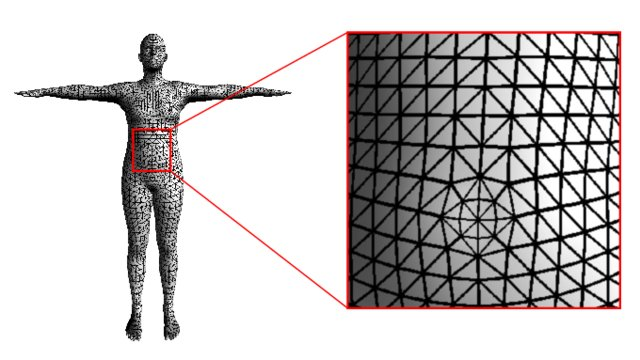
\includegraphics[width=0.6\linewidth]{"../Annexes/Figures/Mesh_model.jpg"}
            \caption{The SMPL mesh model characterizes a human shape. Image from \cite{Wu2020}.}
            \label{fig_meshmodel}
\end{figure}
\FloatBarrier

\vspace*{0.5cm}

\noindent\underline{Machine learning vs. Deep learning:}\\
Machine learning and Deep Learning, as well as Artificial Intelligence, Artificial Neural Networks, or Convolutional Neural Networks, are sometimes used interchangeably. However, they do not exactly refer to the same concepts (Figure~\ref{fig_ai}).\\
\textbf{Artificial Intelligence (AI)} concerns the general concept of machines being able to perform tasks that would seem to require human intelligence, or even to sense, reason, and act accordingly. \\
\textbf{Machine learning (ML)} is a subset of AI, and refers to the concept of machines being able to learn and improve as they are exposed to data. It is a data-driven approach, as opposed to knowledge-driven ones.\\
\textbf{Artificial Neural Networks (ANN)} are a specific way of performing ML, by using a network of units inspired from the natural neuron, and thus mimicking the brain. \\
\textbf{Deep Learning (DL)} refers to an ANN with more than 3 layers of neurons.\\
\textbf{Convolutional Neural Networks (CNN)} are a type of ANN which is particularly suited for image processing.

\begin{figure}[hbtp]
	\centering
            \def\svgwidth{1\columnwidth}
            \fontsize{10pt}{10pt}\selectfont
            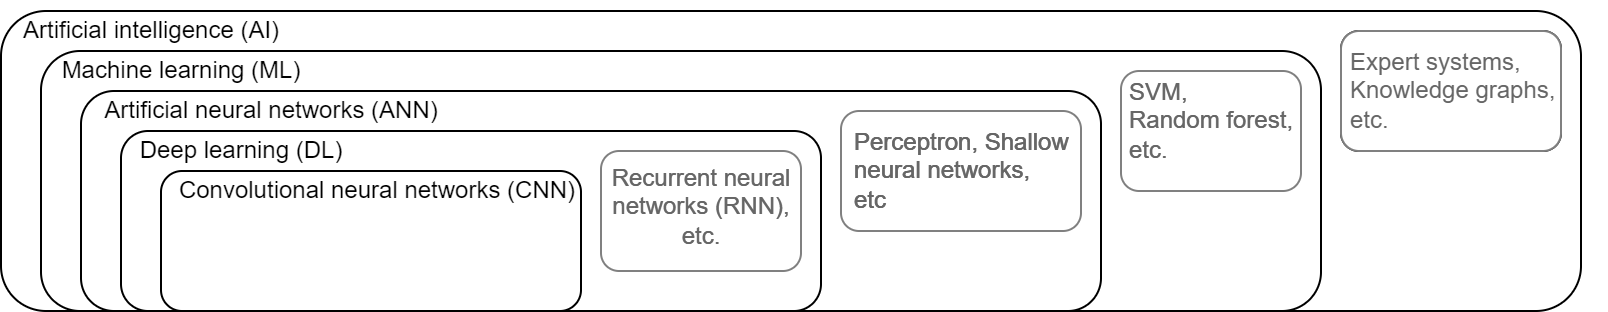
\includegraphics[width=\linewidth]{"../Annexes/Figures/AI_CNN_etc.png"}
            \caption{Diagram of Artificial intelligence, Machine learning, Artificial neural networks, Deep learning, and Convolutional neural networks. The greyed out elements will not be described.}
            \label{fig_ai}
\end{figure}
\FloatBarrier
\vspace*{0.5cm}

\noindent\underline{Dataset vs. Labels: }\\
A \textbf{dataset} is a collection of data used to train a machine learning model. \\
These data need to be labelled prior to training. \textbf{Labels} and \textbf{annotations} can generally be considered as synonyms. Certain datasets come with several kinds of annotations: keypoints, instance segmentation, or image classification for example. Note that a same dataset can be annotated with several keypoint instances, e.g., one focusing on hands, and the other one on the full body.\\
Once labeled, a dataset can be fed to a deep learning \textbf{architecture}, or \textbf{algorithm}, upon which is appended a \textbf{feature extractor}, or \textbf{backbone}, specific to the chosen labelling convention. A \textbf{model} results from this training, which can then be used to predict the labels of new data. Hand-labeled dataset can be used as \textbf{benchmarks} for assessing the model accuracy or speed. \\
In the everyday use, datasets, labeling or annotation, architecture, and models, tend to be used in a confusing way. For instance, the standard OpenPose model has been trained on the COCO and MPII dataset, annotated with COCO, MPII, and additional foot keypoints, on the OpenPose architecture. This results in the OpenPose body\_25 model. 

\vspace*{0.5cm}

\noindent\underline{Single-view vs. Multi-view:}\\
A \textbf{multi-view} (or multiview) system uses several cameras, while a \textbf{single-view}, or \textbf{monocular} one, uses only one. While multi-view systems are always used to infer 3D information, monocular ones can either focus on 2D or 3D information retrieval.\\
\textbf{Single-image}, or \textbf{single-frame} approaches, specifically analyze one single image. In practice, video approaches often perform their analysis image by image.\\

\vspace*{0.5cm}

\noindent\underline{Kinematics vs. Kinetics: }\\
vs dynamics

\vspace*{0.5cm}

\noindent\underline{Spatio-temporal parameters vs Joint kinematics:}\\
both fall under the umbrella of kinematic data. In the customary usage, kinematics describes joint kinematics.

\vspace*{0.5cm}

\noindent\underline{Forward kinematics vs. Direct kinematics:}\\
Forward kinematics: angles -> position
Direct kinematics: position -> angles
analytical solution (direct kinematics, 6DoF) vs. numerical solution (inverse kinematics)





% top-down vs. bottom-up vs. single-person

